% !TeX root = bash.tex
\section{III. Redirect and Pipes}
\begin{frame}
\frametitle{Three Standard Streams}
Every program has three standard streams for I/O:
\vspace{0.3em}

\begin{center}
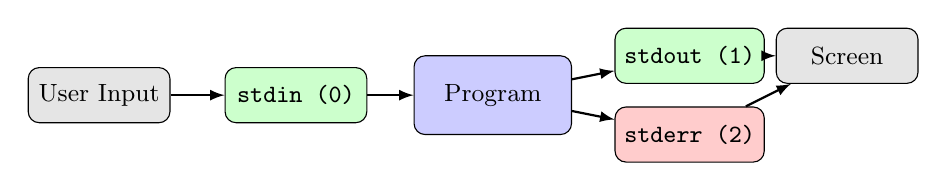
\begin{tikzpicture}[node distance=1.5cm,
    stream/.style={rectangle, draw, fill=green!20, rounded corners, minimum width=1.8cm, minimum height=0.7cm, font=\small},
    prog/.style={rectangle, draw, fill=blue!20, rounded corners, minimum width=2cm, minimum height=1cm, font=\small},
    io/.style={rectangle, draw, fill=gray!20, rounded corners, minimum width=1.8cm, minimum height=0.7cm, font=\small}]
    \node [io] (user) {User Input};
    \node [stream, right of=user, node distance=2.5cm] (stdin) {\tt{stdin} (0)};
    \node [prog, right of=stdin, node distance=2.5cm] (program) {Program};
    \node [stream, right of=program, node distance=2.5cm, yshift=0.5cm] (stdout) {\tt{stdout} (1)};
    \node [stream, right of=program, node distance=2.5cm, yshift=-0.5cm, fill=red!20] (stderr) {\tt{stderr} (2)};
    \node [io, right of=stdout, node distance=2cm] (screen) {Screen};
    
    \draw [-latex, thick] (user) -- (stdin);
    \draw [-latex, thick] (stdin) -- (program);
    \draw [-latex, thick] (program) -- (stdout);
    \draw [-latex, thick] (program) -- (stderr);
    \draw [-latex, thick] (stdout) -- (screen);
    \draw [-latex, thick] (stderr) -- (screen);
\end{tikzpicture}
\end{center}
\vspace{0.3em}

\begin{block}{}
    Normally, stdin is tied to user input, stdout and stderr are both printed on the screen. But we could control where the streams flow. 
\end{block}
\end{frame}

\begin{frame}[fragile]
\frametitle{Redirect stdin (\tt{<})}
You can redirect stdin to read from a file instead of user input.
Try this in \tt{03-pipes/}:
\begin{lstlisting}[language=bash]
$ wc -l              # waits for your input (Ctrl+D to end)
$ wc -l < numbers    # reads from file instead
\end{lstlisting}
\begin{figure}
    \centering
    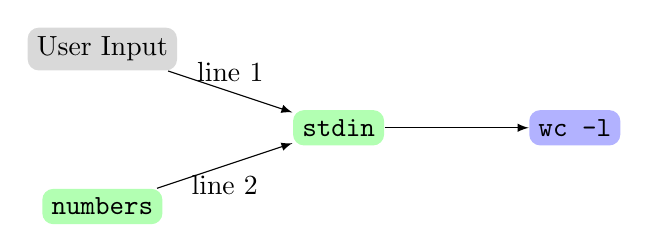
\begin{tikzpicture}
        \tikzstyle{every node}=[rounded corners]
        \node[fill=gray!30]  (input)    at (0,  1) {User Input};
        \node[fill=green!30] (file)     at (0, -1) {\tt{numbers}};
        \node[fill=green!30] (stdin)    at (3,  0) {\tt{stdin}};
        \node[fill=blue!30]  (prog)     at (6,  0) {\tt{wc -l}};
        \tikzstyle{every node}=[fill=none]
        \draw[-latex] (input) -- (stdin) node[above,midway] {line 1};
        \draw[-latex] (file) -- (stdin) node[below,midway] {line 2};
        \draw[-latex] (stdin) -- (prog);
    \end{tikzpicture}
\end{figure}
\end{frame}

\begin{frame}[fragile]
\frametitle{Redirect stdout (\tt{>})}
You can redirect the stdout of a command to a file.
Try this:
\begin{lstlisting}[language=bash]
$ echo hello        # print to terminal
$ echo hello > out  # write to file
\end{lstlisting}
\begin{figure}
    \centering
    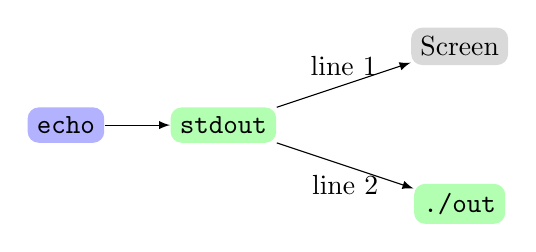
\begin{tikzpicture}
        \tikzstyle{every node}=[rounded corners]
        \node[fill=blue!30]  (prog)        at (0,  0) {\tt{echo}};
        \node[fill=green!30] (stdout)      at (2,  0) {\tt{stdout}};
        \node[fill=gray!30]  (term)        at (5,  1) {Screen};
        \node[fill=green!30] (stdout-file) at (5, -1) {\tt{./out}};
        \tikzstyle{every node}=[fill=none]
        \draw[-latex] (prog) -- (stdout);
        \draw[-latex] (stdout) -- (term) node[above,midway] {line 1};
        \draw[-latex] (stdout) -- (stdout-file) node[below,midway] {line 2};
    \end{tikzpicture}
\end{figure}
\end{frame}

\begin{frame}[fragile]
\frametitle{\tt{>} and \tt{>>}}
Try \tt{>>} instead of \tt{>}. What happens?
\begin{lstlisting}[language=bash]
$ echo hello >> out
$ cat out
\end{lstlisting}
Repeat a few times with both \tt{>} and \tt{>>}. What's the difference?
\pause
\begin{block}{Observation}
    \tt{>} overwrites the file, but \tt{>>} appends to it.
\end{block}
\end{frame}

\begin{frame}[fragile]
\frametitle{Redirect stderr}
\begin{block}{}
To redirect stderr, simply add a `2', and you will get \tt{2>} and \tt{2>>}. Others are the same. 
\end{block}
\begin{block}{}
Besides, \tt{\&>} and \tt{\&>>} means to redirect both stdout and stderr. 
\end{block}
\end{frame}

\begin{frame}[fragile]
\frametitle{Summary of \tt{<} and \tt{>}}
\begin{itemize}
    \item The file must be placed to the right of the redirection operator.
    \item Redirect means to connect a stream to a file. 
\end{itemize}
\end{frame}

\begin{frame}[fragile]
\frametitle{pipes}
Aside from \textbf{connecting streams of one program to files}, we could also connect streams of different programs together \textbf{(stdin to stdout)}.
\vspace{0.5em}

Try this in \tt{03-pipes/}:
\begin{lstlisting}[language=bash]
$ ls random/ | head -n 5
\end{lstlisting}
\begin{figure}
    \centering
    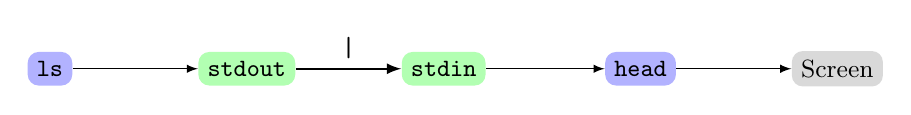
\begin{tikzpicture}
        \tikzstyle{every node}=[rounded corners, font=\small]
        \node[fill=blue!30]  (ls)      at (0,   0) {\tt{ls}};
        \node[fill=green!30] (stdout)  at (2.5, 0) {\tt{stdout}};
        \node[fill=green!30] (stdin)   at (5,   0) {\tt{stdin}};
        \node[fill=blue!30]  (head)    at (7.5, 0) {\tt{head}};
        \node[fill=gray!30]  (screen)  at (10,  0) {Screen};
        \tikzstyle{every node}=[fill=none]
        \draw[-latex] (ls) -- (stdout);
        \draw[-latex, thick] (stdout) -- (stdin) node[above,midway] {\tt{|}};
        \draw[-latex] (stdin) -- (head);
        \draw[-latex] (head) -- (screen);
    \end{tikzpicture}
\end{figure}
\pause
\begin{block}{Observation}
    Normally \tt{head} expects a filename, but when none is given, it
    falls back to stdin — which is what \tt{ls} printed to stdout.
\end{block}

\end{frame}

\begin{frame}[fragile]
\frametitle{The power of pipes}
You can chain commands with pipes. Classic recipe (still in \tt{03-pipes}):
\begin{lstlisting}[language=bash]
$ cat numbers
$ cat numbers | sort
$ cat numbers | sort | uniq
$ cat numbers | sort | uniq | wc -w
\end{lstlisting}
\pause
\begin{block}{Observations}
    \begin{itemize}
        \item Each program takes the last one's stdout as stdin
        \item Only the final program will print to terminal
    \end{itemize}
\end{block}
\begin{block}{Explanation}
    \begin{itemize}
        \item \tt{cat numbers} — print file contents
        \item \tt{sort} — sort lines alphabetically
        \item \tt{uniq} — remove duplicate lines
        \item \tt{wc -w} — count words
    \end{itemize}
\end{block}
\end{frame}

\begin{frame}[fragile]
\frametitle{grep}
Try this in \tt{03-pipes}:
\footnote{For Mac users, instead of \tt{grep} you might have to type \tt{ggrep}}
\begin{lstlisting}[language=bash]
$ ls random/ | grep A+
\end{lstlisting}
\pause
\begin{block}{Explanation}
    \tt{grep} is a powerful tool to match a substring. By default, it takes
    a file (or stdin), and prints all lines containing a pattern (``A+'').
\end{block}
\end{frame}

\begin{frame}
\frametitle{Challenge}
Inside \tt{03-pipes/random/}:
\begin{itemize}
    \item List all filenames containing ``FDU''
    \item List all filenames containing ``UM'' (upper and lower cases)
    \item List all filenames containing ``UM'' but not ``FDU''
        (upper and lower cases for both substrings)
\end{itemize}
\begin{block}{Hint}
    \cverb|-i| to make \cverb|grep| case-insensitive, \cverb|-v| for negation.
\end{block}
\end{frame}

\begin{frame}[fragile]
\frametitle{Solution}
\begin{lstlisting}[language=bash]
$ ls | grep FDU
$ ls | grep -i UM
$ ls | grep -i UM | grep -i -v FDU
\end{lstlisting}
\end{frame}

\begin{frame}
\frametitle{Conclusion}
\begin{itemize}
    \item Files and directories form a tree
    \item One tool does one thing, but flags specify how
    \item When in doubt, read documentation
    \item Chain together tools and unleash immense power
\end{itemize}
\end{frame}
